% ##################################################################################################################
\section{New York City}
\label{sec:nyc}
\hfill \textbf{Author:} Christoph Dobler

% ##################################################################################################################
The \gls{matsim} model of New York is an example of an agent-based model based on the outcome of a given activity-based demand generation process. In this case the \gls{nybpm} of Parson Brinkerhoff \citep[][]{VovshaEtAl_TRR_2002, ParsonsBrinckerhoff_ResRep_NYBPM_2005, ParsonsBrinckerhoff_ResRep_NYBPM_2009}. It produces persons with individual activity chains. \gls{matsim} is chosen as the simulation based alternative of conventional assignment processes.

Activity locations are selected on zonal level (3\,824\,zones), timings (i.e.,\,start time and duration) are chosen using given distributions. As part of the conversion process to \gls{matsim}, locations were distributed within the zones according to land use and buildings. For the route assignment, transport modes were converted into ones supported by \gls{matsim}. The resulting population contained 5.3\,million persons (25\,\% sample).

A \gls{multimodal} network was creating containing car and public transport links was created for the \gls{matsim} model. Car links were derived from network data from the aggregated model including capacity, number of lanes and speed limit. For the public transport network, a shape file containing the routes of all lines was available. After converting and cleaning the data, the final multi-modal network contained 498\,000 nodes and 541\,000 links. Based on further public transport related data, a full schedule was created including different public transport modes (bus, train, etc.).

An example for the outcomes of the final model is shown in Figure~\ref{fig:ny_car_share_full} and Figure~\ref{fig:ny_car_share_gross}. They depict the car share of all performed trips within a certain region. Red indicates a high share, blue a low one. In Figure~\ref{fig:ny_car_share_full} the trips are aggregated on zonal level. In Figure \ref{fig:ny_car_share_gross}, the high resolution of the \gls{matsim} model is shown: there, the trips are aggregated not on zonal level but by using hexagons with a side length of 500\,meters.

\createfigure%
{Car share (entire modeled area)}%
{Car share (entire modeled area)}%
{\label{fig:ny_car_share_full}}%
{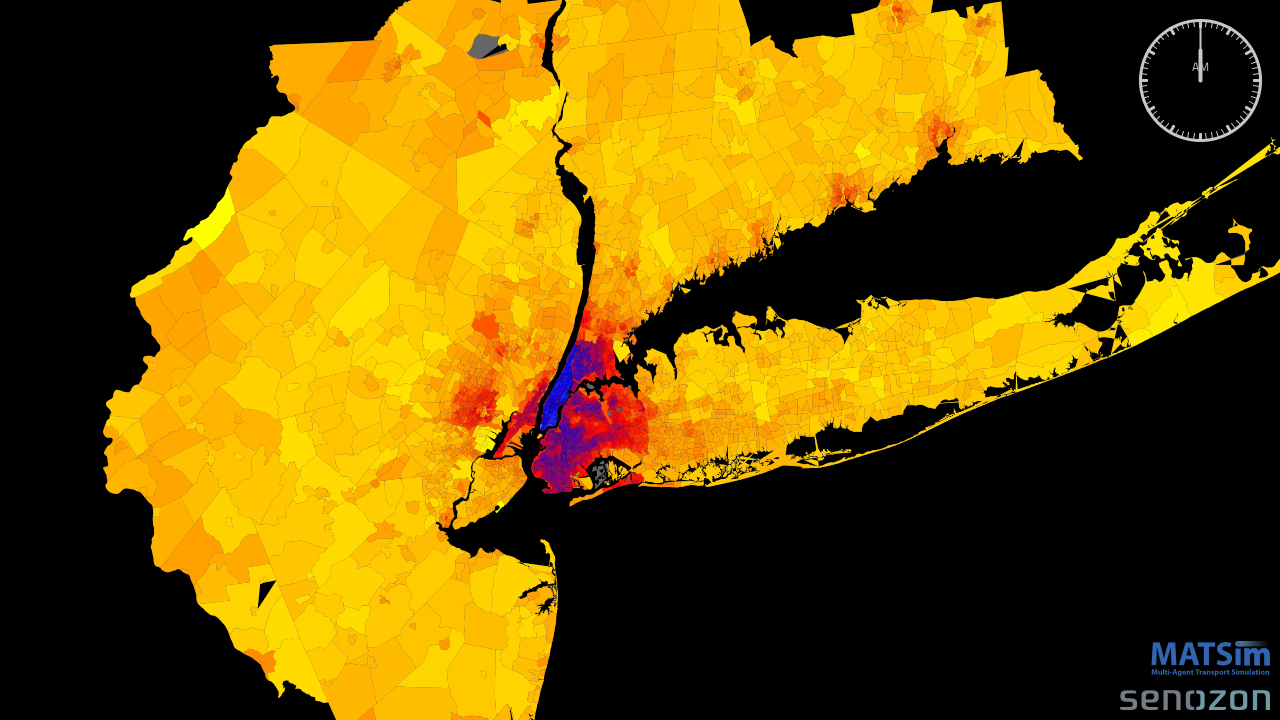
\includegraphics[width=0.95\textwidth, angle=0]{./using/figures/ny_carshare_TAZ_full.png}}%
{}

\createfigure%
{Car share (Manhattan)}%
{Car share (Manhattan)}%
{\label{fig:ny_car_share_gross}}%
{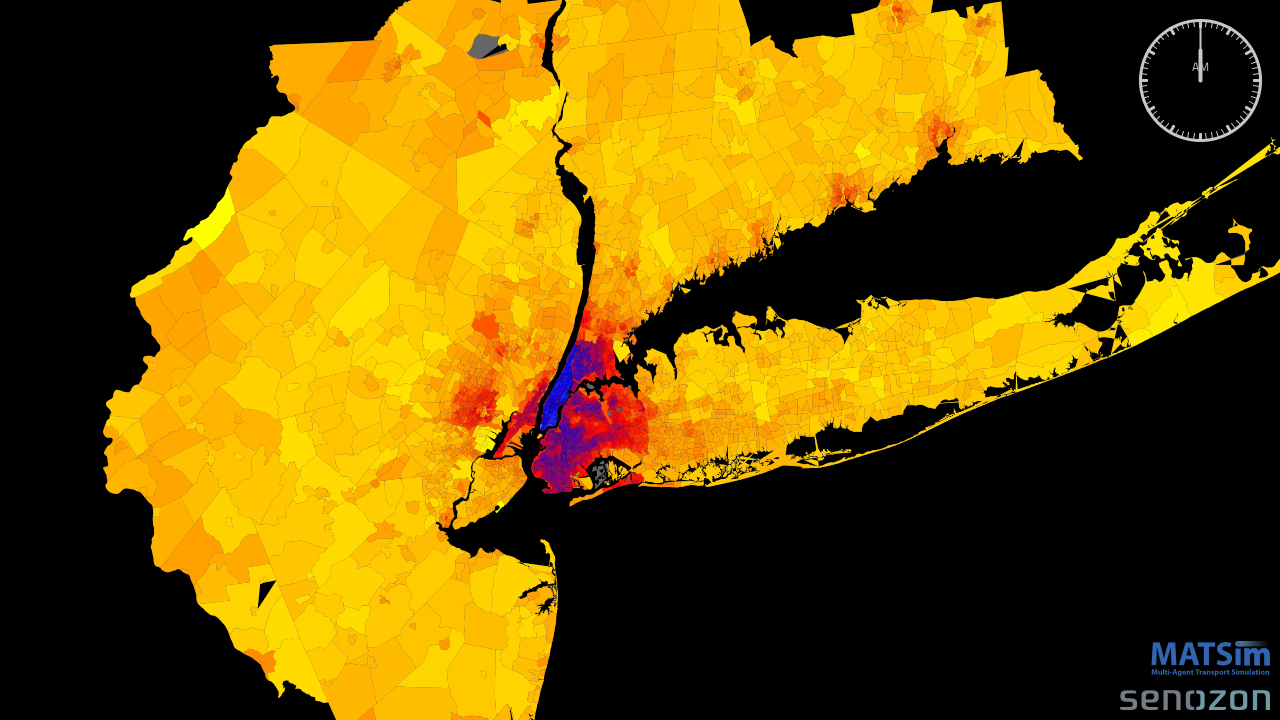
\includegraphics[width=0.95\textwidth, angle=0]{./using/figures/ny_carshare_TAZ_full.png}}%
{}

Finally, Figure~\ref{fig:ny_traffic} shows the traffic flows in Lower Manhattan. Cars are represented by rectangulars, public transport vehicles by arrows. Further outcomes of the model are presented by \citet[][]{Balmer_unpub_ZMNY_2014}. A movie can be found online at \url{http://senozon.com/news/2014-05/zürich-meets-new-york}

\createfigure%
{Traffic flows in Lower Manhattan}%
{Traffic flows in Lower Manhattan}%
{\label{fig:ny_traffic}}%
{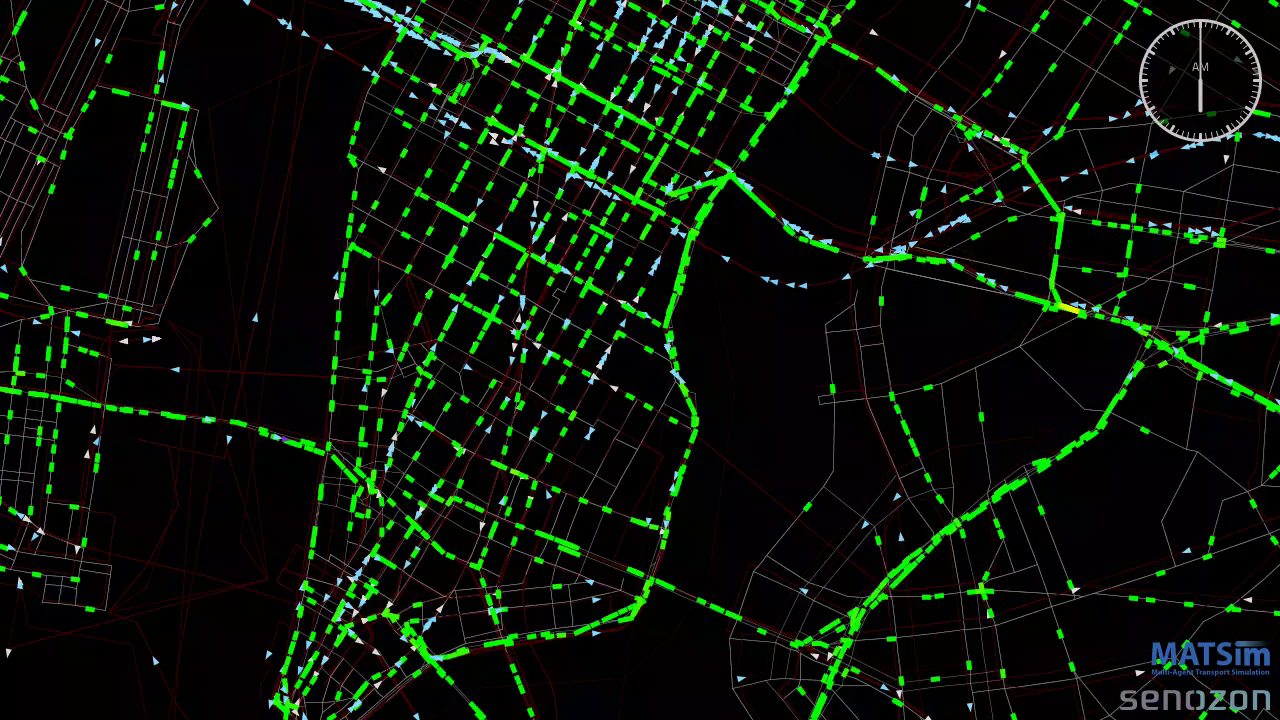
\includegraphics[width=0.95\textwidth, angle=0]{./using/figures/ny_traffic.png}}%
{}

% ##################################################################################################################